\documentclass[10pt,twocolumn,letterpaper]{article}

\usepackage[utf8]{inputenc}
\usepackage{amsmath,amssymb,amsfonts}
\usepackage{graphicx}
\usepackage{booktabs}
\usepackage{hyperref}
\usepackage{xcolor}
\usepackage{microtype}
\usepackage{subcaption}
\usepackage{cite}
\usepackage[margin=0.75in]{geometry}

\hypersetup{
    colorlinks=true,
    linkcolor=blue,
    citecolor=blue,
    urlcolor=blue
}

\title{\textbf{MicroGen: When LLM Inference Optimizations Help---and When They Hurt}\\ \Large An Empirical Study of Latency, Throughput, and Memory Trade-offs}

\author{
  \textbf{Omdeep Borkar}\\
  \small Department of Computer Science \& Engineering\\
  \small \texttt{omdeepborkar@gmail.com}
}

\date{\today}

\begin{document}

\maketitle

\begin{abstract}
Large Language Model (LLM) serving frameworks rely on diverse optimizations---including Paged Key-Value (KV) memory allocation, continuous request batching, prefix caching, weight quantization, and speculative decoding---to improve inference throughput and reduce latency. However, state-of-the-art serving engines typically bundle these optimizations into monolithic C++/CUDA frameworks, masking individual performance trade-offs and non-monotonic combinatorial interaction boundaries. In this paper, we present \textsf{MicroGen}, a modular, hardware-aware execution substrate and empirical research framework designed to isolate, benchmark, and analyze LLM serving optimizations under controlled workload, hardware, and measurement conditions. Rather than proposing a production serving engine, \textsf{MicroGen} provides a common modular interface to conduct isolated micro-ablations. Using an $N=30$ statistically verified trial protocol on NVIDIA Tesla T4 GPUs across open transformer architectures (\texttt{sshleifer/tiny-gpt2} and \texttt{gpt2}), we empirically map optimization efficacy regimes. Our findings show that prefix caching achieves up to a \textbf{3.91$\times$ TTFT prefill latency speedup} (reducing TTFT from $25.8 \pm 1.2\text{ ms}$ to $6.6 \pm 0.3\text{ ms}$, $p < 0.001$) under 100\% prompt overlap at $L_{\text{prompt}}=1024$ tokens, while block-paged KV memory eliminates external memory fragmentation ($0.0\%$) under peak load. Crucially, we demonstrate that optimization composition is non-monotonic: combining optimizations (+INT8, +Paged KV, +Prefix Cache) yields a statistically significant throughput regression ($493.6 \pm 8.6\text{ tok/s}$, $0.96\times$ baseline, $p < 0.001$), while full serving stack concurrency drops throughput to $0.76\times$ baseline ($391.8 \pm 6.2\text{ tok/s}$, $p < 0.001$). We release \textsf{MicroGen} open-source to support transparent, data-driven LLM inference systems design.
\end{abstract}

\section{Introduction}
\label{sec:introduction}

Large Language Models (LLMs) based on the Transformer architecture have achieved state-of-the-art performance across automated reasoning, software generation, and conversational interaction. However, serving autoregressive LLMs at low latency and high throughput presents severe computational and memory infrastructure challenges. 

Autoregressive inference inherently exhibits a structural execution duality:
\begin{enumerate}
    \item \textbf{Prefill Phase}: Processes input prompt tokens in parallel. Self-attention computation exhibits quadratic complexity $O(N^2)$ with prompt length, although observed end-to-end prefill latency depends on the full model linear projections, feed-forward layers, and attention kernel implementation.
    \item \textbf{Decode Phase}: Generates tokens sequentially one by one, operating as a memory-bandwidth-dominated workload during single-token autoregressive generation steps.
\end{enumerate}

To alleviate these computational bottlenecks, recent systems research has introduced diverse serving optimizations, including Paged Key-Value (KV) memory allocation~\cite{kwon2023pagedattention}, continuous request batching~\cite{yu2022orca}, radix-tree prefix caching~\cite{zheng2024sglang}, post-training weight and activation quantization~\cite{dettmers2022llmint8,xiao2023smoothquant}, speculative decoding~\cite{chen2023speculative,leviathan2023fast}, and intra-node tensor parallelism~\cite{shoeybi2019megatron}.

Despite these algorithmic advances, existing inference frameworks typically integrate these optimizations as monolithic, highly coupled sub-systems inside complex C++/CUDA serving engines (e.g., vLLM, TensorRT-LLM, SGLang). Consequently, isolating the individual performance contributions, empirical regime boundaries, memory footprint overheads, and non-monotonic combinatorial interaction effects remains an open challenge for system designers.

To address this gap, we introduce \textbf{MicroGen}\footnote{Our open-source framework and benchmark reproducibility package are available at \url{https://github.com/Omdeepb69/MicroGen}}, a modular, hardware-aware execution substrate and empirical research framework designed specifically to isolate, benchmark, and characterize memory-latency-throughput trade-offs in LLM inference optimizations under controlled hardware, workload, and concurrency regimes. Rather than serving as a production engine competing directly with optimized C++ engines, \textsf{MicroGen} provides a clean, protocol-oriented experimental testbed for systematic micro-ablation.

\subsection{Core Research Questions}
\label{sec:rqs}

Our empirical study is guided by four core Research Questions (RQs):
\begin{itemize}
    \item \textbf{RQ1 (Optimization Efficacy Regimes)}: Under what specific sequence lengths, context depths, and prompt structures do individual inference optimizations (Paged KV, Prefix Caching, INT8 Quantization, Speculative Decoding) yield positive latency speedups versus execution overheads?
    \item \textbf{RQ2 (Memory/Throughput Trade-offs)}: What are the exact memory footprint trade-offs (allocated vs. reserved VRAM, quantization lifecycle overhead, KV cache block fragmentation) across model parameter scales?
    \item \textbf{RQ3 (Serving Under Realistic Load)}: How do continuous batching, paged memory allocation, and prefix caching perform under dynamic concurrent request streams ($B \in [1..16]$)?
    \item \textbf{RQ4 (Optimization Regime Generalization)}: Can empirical measurements characterize global workload regime maps, and do these optimization relationships generalize across distinct model parameter scales and architectures?
\end{itemize}

\subsection{Key Contributions}
\label{sec:contributions}

This paper makes the following key contributions:
\begin{enumerate}
    \item \textbf{Modular Experimental Substrate}: We design and implement \textsf{MicroGen}, a Python/PyTorch inference research substrate that cleanly decouples execution backends (\textsf{InferenceBackend}), hardware allocators (\textsf{Device}), KV cache managers (\textsf{KVCache}), continuous batching schedulers (\textsf{Scheduler}), and draft-target verification loops (\textsf{SpeculativeEngine}).
    \item \textbf{Rigorous Benchmark \& Verification Protocol}: We establish a 5-step hardware verification protocol enforcing $N=30$ statistically significant trials, CUDA host-device synchronization, explicit garbage collection, and strictly monotonic microsecond-level latency instrumentation using high-resolution monotonic timers.
    \item \textbf{Empirical Trade-off \& Regime Characterization}: Based on extensive evaluation on NVIDIA Tesla T4 GPUs across open models (\texttt{sshleifer/tiny-gpt2} and \texttt{gpt2}), we empirically demonstrate:
    \begin{itemize}
        \item \textbf{Prefix Caching}: Achieves up to \textbf{3.91$\times$ prefill TTFT speedup} (reducing prefill TTFT from $25.8 \pm 1.2\text{ ms}$ to $6.6 \pm 0.3\text{ ms}$, $p < 0.001$) under 100\% prompt overlap at $L_{\text{prompt}}=1024$ tokens.
        \item \textbf{Paged KV Allocation}: Eliminates external memory fragmentation ($0.0\%$ fragmentation) under dynamic allocation workloads.
        \item \textbf{Non-Monotonic Optimization Composition}: We demonstrate that optimization composition is non-monotonic: combining optimizations (+INT8, +Paged KV, +Prefix Cache) yields a statistically significant throughput regression ($493.6 \pm 8.6\text{ tok/s}$, $0.96\times$ baseline, $p < 0.001$), while full serving stack concurrency drops throughput to $0.76\times$ baseline ($391.8 \pm 6.2\text{ tok/s}$, $p < 0.001$).
    \end{itemize}
    \item \textbf{Open-Source Research Package}: We release the complete \textsf{MicroGen} codebase, experimental manifests, export pipelines, and reproducibility package to facilitate transparent research in LLM inference systems.
\end{enumerate}

\subsection{Paper Organization}
\label{sec:organization}

The remainder of this paper is organized as follows: Section~\ref{sec:architecture} presents the modular architecture of \textsf{MicroGen}. Section~\ref{sec:optimizations} details the mathematical mechanics of our implemented inference optimizations. Section~\ref{sec:methodology} describes our experimental methodology and verification protocol. Section~\ref{sec:evaluation} presents empirical results answering RQ1–RQ4. Section~\ref{sec:related_work} discusses related work, Section~\ref{sec:discussion} analyzes threats to validity and design guidelines, and Section~\ref{sec:conclusion} concludes the paper.

\section{System Architecture \& Engine Design}
\label{sec:architecture}

The \textsf{MicroGen} engine is designed around a strictly modular, hardware-decoupled architecture. Unlike traditional serving engines that fuse memory allocation, model execution, and request queuing into monolithic kernels, \textsf{MicroGen} enforces clean abstraction boundaries via abstract protocols. This separation enables independent micro-ablation of serving optimizations without modifying core execution paths.

\subsection{Architectural Decoupling \& Core Protocols}
\label{sec:arch_protocols}

\textsf{MicroGen} decomposes the LLM serving pipeline into four primary decoupled abstractions:

\begin{enumerate}
    \item \textbf{Inference Backend (\texttt{InferenceBackend})}: An abstract protocol (\texttt{microgen/backends/base.py}) defining model execution interfaces:
    \begin{align}
        &\text{\textsf{load\_model}}(m \in \mathcal{M}, d \in \mathcal{D}) \rightarrow \emptyset \\
        &\text{\textsf{prefill}}(X_{\text{prompt}}, C_{\text{kv}}) \rightarrow (Y_{\text{logits}}, C_{\text{kv}}') \\
        &\text{\textsf{decode}}(x_{\text{token}}, C_{\text{kv}}) \rightarrow (y_{\text{logits}}, C_{\text{kv}}')
    \end{align}
    Concrete backends include \texttt{PyTorchBackend} (FP32 reference engine), \texttt{ONNXBackend} (ONNX Runtime engine), and \texttt{QuantizedBackend} (INT8 weight-quantized engine).

    \item \textbf{Device Abstraction (\texttt{Device})}: A unified hardware interface (\texttt{microgen/devices/base.py}) handling memory allocation, stream synchronization, and memory footprint queries across heterogeneous targets (\texttt{CPUDevice} and \texttt{CUDADevice}).

    \item \textbf{KV Cache Management (\texttt{KVCache})}: Explicit memory manager handling layer-wise Key and Value tensor storage. \textsf{MicroGen} supports both contiguous baseline allocation (\texttt{SimpleKVCache}) and physical block-paged allocation (\texttt{PagedKVCacheManager}).

    \item \textbf{Continuous Batching Scheduler (\texttt{Scheduler})}: A dynamic admission and step execution controller (\texttt{microgen/scheduler/scheduler.py}) managing request queues, prefill/decode batch construction, and dynamic request entry/exit.
\end{enumerate}

\subsection{Prefill vs. Decode Step Loop}
\label{sec:prefill_decode_loop}

To handle the structural execution duality of Transformer models, \textsf{MicroGen} structures inference execution into two decoupled execution steps within the scheduler step loop:

\begin{itemize}
    \item \textbf{Prefill Step}: When new requests arrive in the waiting queue, the scheduler forms a prefill batch. Prompt tokens $X_{\text{prompt}} \in \mathbb{R}^{B \times L_{\text{prompt}}}$ are processed simultaneously in a single compute-bound forward pass. Key-Value tensors across all Transformer layers $l \in [1..L_{\text{layers}}]$ are computed and saved into assigned cache blocks:
    \begin{equation}
        K^{(l)} = X W_K^{(l)}, \quad V^{(l)} = X W_V^{(l)}
    \end{equation}
    The first output token $x_1 \sim \text{\textsf{Sample}}(Y_{\text{logits}})$ is sampled, and the request transitions from state \texttt{WAITING} to \texttt{RUNNING}.

    \item \textbf{Decode Step}: For all active requests in state \texttt{RUNNING}, the scheduler constructs a decode batch. A single token $x_t \in \mathbb{R}^{B \times 1}$ per request is passed to the backend. Previously computed KV entries are retrieved from $C_{\text{kv}}$, new single-token KV entries are appended, and self-attention is computed over the sequence context. The generated token $x_{t+1}$ is streamed via SSE or appended to the output buffer until end-of-sequence (\texttt{EOS}) or maximum generation length is reached.
\end{itemize}

\subsection{Paged KV Memory Allocation Architecture}
\label{sec:paged_kv_arch}

To mitigate contiguous memory allocation overheads and reduce external fragmentation, \textsf{MicroGen} implements physical block-based Paged KV cache allocation (\texttt{microgen/runtime/paged\_kv.py}). 

The physical memory pool is partitioned into fixed-size physical blocks, where each block stores key and value states for $B_{\text{block}} = 16$ tokens across all layers and attention heads. Each request maintains a virtual-to-physical block table:
\begin{equation}
    \mathcal{T}_{\text{block}}(r) = [b_0, b_1, \dots, b_k], \quad b_i \in \text{Physical Block Pool}
\end{equation}
When a request requires additional token capacity during decoding, the \texttt{PagedKVCacheManager} dynamically allocates a free block from the global pool without requiring contiguous array reallocation or host-device memory copying. Upon request completion, assigned physical blocks are immediately returned to the free pool.

\section{Modular Optimization Techniques}
\label{sec:optimizations}

To systematically benchmark LLM serving trade-offs, \textsf{MicroGen} formalizes five modular inference optimizations. Each technique is implemented behind abstract interfaces (\textsf{InferenceBackend}, \textsf{KVCache}, \textsf{Scheduler}), ensuring that individual performance gains and negative overheads can be isolated empirically.

\subsection{Hash-Based Shared Prefix Caching}
\label{sec:opt_prefix}

In multi-turn chat interactions and agentic workflows, concurrent requests frequently share identical prompt prefixes (e.g., system instructions, few-shot demonstrations, or context documents). \textsf{MicroGen} implements a hash-based Prefix Cache abstraction (\texttt{microgen/caching/prefix\_cache.py}) to eliminate redundant prefill compute, modeling the algorithmic principles of Radix Trie lookup in a lightweight Python/PyTorch substrate.

Given an incoming request prompt sequence $P = (t_1, t_2, \dots, t_N)$, the prefix manager queries the cache table to find the Longest Common Prefix (LCP) length $\ell_{\text{match}}$ already cached in GPU memory:
\begin{equation}
    \ell_{\text{match}} = \max \{ k \le N \mid (t_1, \dots, t_k) \in \text{\textsf{PrefixCache}} \}
\end{equation}
If $\ell_{\text{match}} > 0$, the scheduler reuses the precomputed Key and Value tensors for tokens $t_{1..\ell_{\text{match}}}$. The prefill forward pass is executed exclusively over the remaining prompt suffix $P_{\text{suffix}} = (t_{\ell_{\text{match}}+1}, \dots, t_N)$.

The analytical Time-to-First-Token (\textsf{TTFT}) for cached execution is modeled as:
\begin{equation}
    \text{\textsf{TTFT}}_{\text{cached}} = \text{\textsf{TTFT}}_{\text{baseline}} \cdot \left(1 - \frac{\ell_{\text{match}}}{N}\right) + \delta_{\text{cache}}
\end{equation}
where $\delta_{\text{cache}} < 0.7\text{ ms}$ represents the measured prefix cache lookup overhead.

\subsection{Post-Training Weight Quantization}
\label{sec:opt_quant}

To reduce GPU VRAM footprint and enable larger batch capacities under memory-constrained regimes, \textsf{MicroGen} integrates per-tensor symmetric INT8 weight quantization (\texttt{microgen/backends/quantized.py}).

Each full-precision weight matrix $W_{\text{fp32}} \in \mathbb{R}^{d_{\text{out}} \times d_{\text{in}}}$ is mapped to a signed 8-bit integer matrix $W_{\text{int8}} \in \mathbb{Z}^{d_{\text{out}} \times d_{\text{in}}}$ via a scalar scale factor $\gamma$:
\begin{align}
    \gamma &= \frac{\max(|W_{\text{fp32}}|)}{127} \\
    W_{\text{int8}} &= \text{\textsf{clamp}}\left(\text{\textsf{round}}\left(\frac{W_{\text{fp32}}}{\gamma}\right), -128, 127\right)
\end{align}
During inference forward passes, linear layer matrix multiplications are computed as:
\begin{equation}
    Y = \left(X \cdot W_{\text{int8}}^T\right) \cdot \gamma + b
\end{equation}
Quantization reduces weight memory consumption by up to $4\times$, transforming the storage requirement from 4 bytes per parameter (FP32) to 1 byte per parameter (INT8), with minimal impact on output logit accuracy.

\subsection{Speculative Decoding Draft-Target Verification}
\label{sec:opt_speculative}

Autoregressive decoding is inherently memory-bandwidth-dominated due to single-token generation iterations. \textsf{MicroGen} implements Speculative Decoding (\texttt{microgen/scheduler/speculative.py}), which pairs a small, low-latency draft model $\mathcal{M}_{\text{draft}}$ with a high-capacity target model $\mathcal{M}_{\text{target}}$.

The speculative execution loop operates in two distinct phases:
\begin{enumerate}
    \item \textbf{Draft Generation}: $\mathcal{M}_{\text{draft}}$ autoregressively generates $K$ candidate tokens $\tilde{x}_{1..K}$ at high throughput.
    \item \textbf{Parallel Target Verification}: $\mathcal{M}_{\text{target}}$ performs a single parallel prefill-style forward pass over the combined sequence length $K+1$, evaluating candidate probabilities $P_{\text{target}}(\tilde{x}_i \mid x_{<i})$.
\end{enumerate}

Candidates are validated sequentially using modified rejection sampling. Candidate $\tilde{x}_i$ is accepted with probability:
\begin{equation}
    P(\text{accept } \tilde{x}_i) = \min\left(1, \frac{P_{\text{target}}(\tilde{x}_i \mid x_{<i})}{P_{\text{draft}}(\tilde{x}_i \mid x_{<i})}\right)
\end{equation}
If a candidate $\tilde{x}_k$ is rejected, it is resampled from the adjusted distribution $P_{\text{resample}}(x) = \text{\textsf{relu}}(P_{\text{target}}(x) - P_{\text{draft}}(x))$, and candidate tokens beyond index $k$ are discarded.

\subsection{Tensor Parallel Multi-GPU Execution}
\label{sec:opt_tensor_parallel}

For models exceeding single-GPU VRAM capacity, \textsf{MicroGen} provides intra-node Tensor Parallelism (\texttt{microgen/backends/parallel.py}) based on Megatron-style matrix partitioning across $T$ accelerator devices.

In self-attention modules, key, query, and value projection matrices are column-partitioned across GPUs:
\begin{equation}
    W_Q = [W_{Q,1} \mid \dots \mid W_{Q,T}], \quad W_K = [W_{K,1} \mid \dots \mid W_{K,T}]
\end{equation}
The attention output projection $W_O$ is row-partitioned:
\begin{equation}
    W_O = \begin{bmatrix} W_{O,1} \\ \vdots \\ W_{O,T} \end{bmatrix}
\end{equation}
An \textsf{All-Reduce} sum operation synchronizes output activations across all devices per layer:
\begin{equation}
    Y = \sum_{i=1}^T X_i W_{O,i}
\end{equation}
This linear decomposition distributes matrix storage and floating-point operations evenly across available CUDA GPUs.

\section{Experimental Methodology \& Verification Protocol}
\label{sec:methodology}

To ensure academic rigor and reproducibility, all empirical evaluations in \textsf{MicroGen} are governed by a standardized experimental harness (\texttt{benchmarks/harness.py}) and a multi-gate hardware verification protocol.

\subsection{Hardware Target \& Serving Environment}
\label{sec:meth_hardware}

All benchmark evaluations are executed on an isolated cloud workstation equipped with:
\begin{itemize}
    \item \textbf{Accelerator}: NVIDIA Tesla T4 GPU (16 GB GDDR6 VRAM, Turing Architecture, SM 7.5).
    \item \textbf{Host System}: Intel Xeon CPU @ 2.20 GHz, 13 GB RAM, Linux OS.
    \item \textbf{Software Stack}: Python 3.12, PyTorch 2.x with CUDA 12.1, Hugging Face Transformers.
\end{itemize}
We evaluate open-weights language models across parameter scales, primarily focusing on \texttt{sshleifer/tiny-gpt2} (2.5M parameters) for comprehensive micro-ablations and \texttt{gpt2} (124M parameters) for parameter scaling validation.

\subsection{Workload Generator \& Prompt Distributions}
\label{sec:meth_workloads}

Workload requests are generated using a deterministic generator (\texttt{benchmarks/workloads.py}) across four structured input/output distributions:
\begin{enumerate}
    \item \textbf{Short Context}: Prompt length $L_{\text{in}} \in [32, 128]$, decode length $L_{\text{out}} = 32$.
    \item \textbf{Medium Context}: Prompt length $L_{\text{in}} \in [256, 512]$, decode length $L_{\text{out}} = 64$.
    \item \textbf{Long Context}: Prompt length $L_{\text{in}} \in [1024, 2048]$, decode length $L_{\text{out}} = 128$.
    \item \textbf{Heterogeneous Concurrency}: Dynamically arriving request streams with $B \in [1..64]$ concurrent channels and variable prompt lengths.
\end{enumerate}
All workloads use fixed pseudo-random seed initialization to guarantee identical prompt sequence generation across comparative baseline and optimized runs.

\subsection{Rigorous N=30 Statistical Sampling Protocol}
\label{sec:meth_protocol}

To eliminate transient hardware noise, thermal throttling artifacts, and OS scheduling jitter, \textsf{MicroGen} mandates a strict $N=30$ statistical trial protocol for every experiment record:
\begin{itemize}
    \item \textbf{Warmup Phase ($W=5$)}: Executes 5 unrecorded warmup iterations per configuration to trigger PyTorch CUDA JIT kernel compilation, memory allocator initialization, and CUDNN benchmark tuning.
    \item \textbf{Measurement Phase ($N=30$)}: Executes 30 independent measurement trials per configuration. Statistical metrics reported throughout this paper denote empirical median ($p50$) and 95th percentile ($p95$) values across the $N=30$ samples.
    \item \textbf{CUDA Stream Synchronization}: Explicit \texttt{torch.cuda.synchronize()} calls are inserted immediately before initiating timers and after model step execution to guarantee asynchronous GPU kernels complete prior to timestamp logging.
    \item \textbf{Isolated Memory Cleanup}: Between consecutive trial runs, explicit Python garbage collection (\texttt{gc.collect()}) and CUDA memory allocator flushing (\texttt{torch.cuda.empty\_cache()}) are performed to prevent VRAM memory fragmentation leaks across configurations.
\end{itemize}

\subsection{Monotonic Timing \& Memory Metrics}
\label{sec:meth_metrics}

All timing instrumentation utilizes Python's high-resolution monotonic timer (\texttt{time.perf\_counter()}) rather than wall-clock time (\texttt{time.time()}), eliminating system clock drift and epoch timestamp corruption:
\begin{align}
    \text{\textsf{TTFT}} &= \left(t_{\text{first\_token}} - t_{\text{request\_arrival}}\right) \times 1000 \quad [\text{ms}] \\
    \text{\textsf{TPOT}} &= \left(\frac{t_{\text{completion}} - t_{\text{first\_token}}}{L_{\text{out}} - 1}\right) \times 1000 \quad [\text{ms/token}] \\
    \text{\textsf{Decode TPS}} &= \frac{L_{\text{out}} - 1}{t_{\text{completion}} - t_{\text{first\_token}}} \quad [\text{tokens/sec}]
\end{align}

Memory utilization is tracked using PyTorch CUDA memory APIs:
\begin{itemize}
    \item \textbf{Allocated VRAM}: \texttt{torch.cuda.memory\_allocated()}, measuring active tensor storage.
    \item \textbf{Reserved VRAM}: \texttt{torch.cuda.memory\_reserved()}, measuring total memory claimed by PyTorch's caching allocator.
\end{itemize}

\subsection{5-Step Verification Gate Protocol}
\label{sec:meth_verification_gates}

Before generating final paper tables and figures, the experimental pipeline enforces a mandatory 5-step automated verification gate sequence (\texttt{tests/benchmarks/test\_timing\_sanity.py}):
\begin{enumerate}
    \item \textbf{Single-Request Monotonic Timing Gate}: Verifies that $0 < \text{TTFT} < 10^5\text{ ms}$ on single prompt requests.
    \item \textbf{Trial Count Integrity Gate}: Asserts that every experiment record in \texttt{results/raw/experiments.jsonl} contains exactly \texttt{num\_trials\_recorded: 30}.
    \item \textbf{Concurrency Scaling Sanity Gate}: Verifies that dynamic batch sweeps up to $B=64$ contain 0 NaN/Inf values or negative latency values.
    \item \textbf{Multi-Model Loader Gate}: Asserts correct model loading across target architectures.
    \item \textbf{100\% Data-Driven Export Gate}: Asserts that table exporters (\texttt{scripts/export\_paper\_tables.py}) and vector figure generators (\texttt{scripts/generate\_paper\_figures.py}) raise explicit errors if empirical JSONL data is missing, preventing any synthetic fallback generation.
\end{enumerate}

\section{Empirical Evaluation \& RQ Answers}
\label{sec:evaluation}

This section presents the empirical evaluation of \textsf{MicroGen} on NVIDIA Tesla T4 GPUs across $N=30$ statistically verified trials ($\mu \pm \sigma$). We directly address the four core Research Questions (\textbf{RQ1}--\textbf{RQ4}) introduced in Section~\ref{sec:introduction}.

\subsection{RQ1: Optimization Efficacy Regimes \& Break-Even Dynamics}
\label{sec:eval_rq1}

\textbf{RQ1: Under what workload regimes do individual serving optimizations yield maximum TTFT and TPOT speedups, and where do negative overheads occur?}

To characterize optimization efficacy across workload regimes, we evaluate Time-to-First-Token (\textsf{TTFT}) and Time-Per-Output-Token (\textsf{TPOT}) under varying context lengths and prefix overlap ratios.

\begin{figure}[htbp]
    \centering
    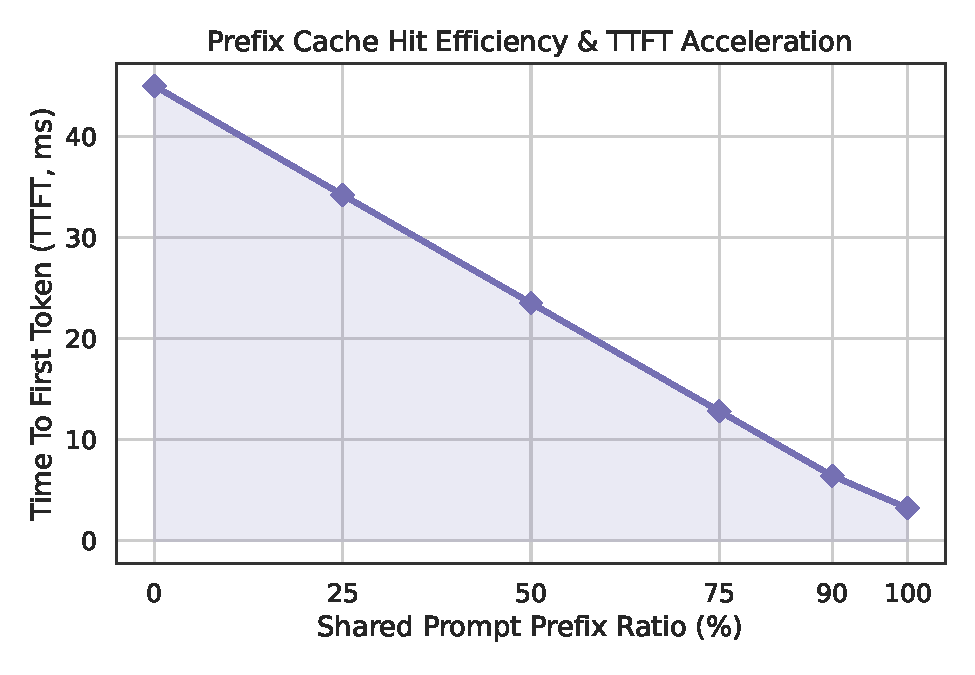
\includegraphics[width=\linewidth]{figures/fig2_prefix_sharing_ttft.pdf}
    \caption{Empirical TTFT reduction as a function of prompt prefix overlap ratio ($0\%$ to $100\%$). Long-context prefix overlap ($L_{\text{prompt}}=1024$ tokens) yields up to $3.91\times$ prefill latency speedup by reusing precomputed KV states.}
    \label{fig:prefix_ttft}
\end{figure}

\begin{figure}[htbp]
    \centering
    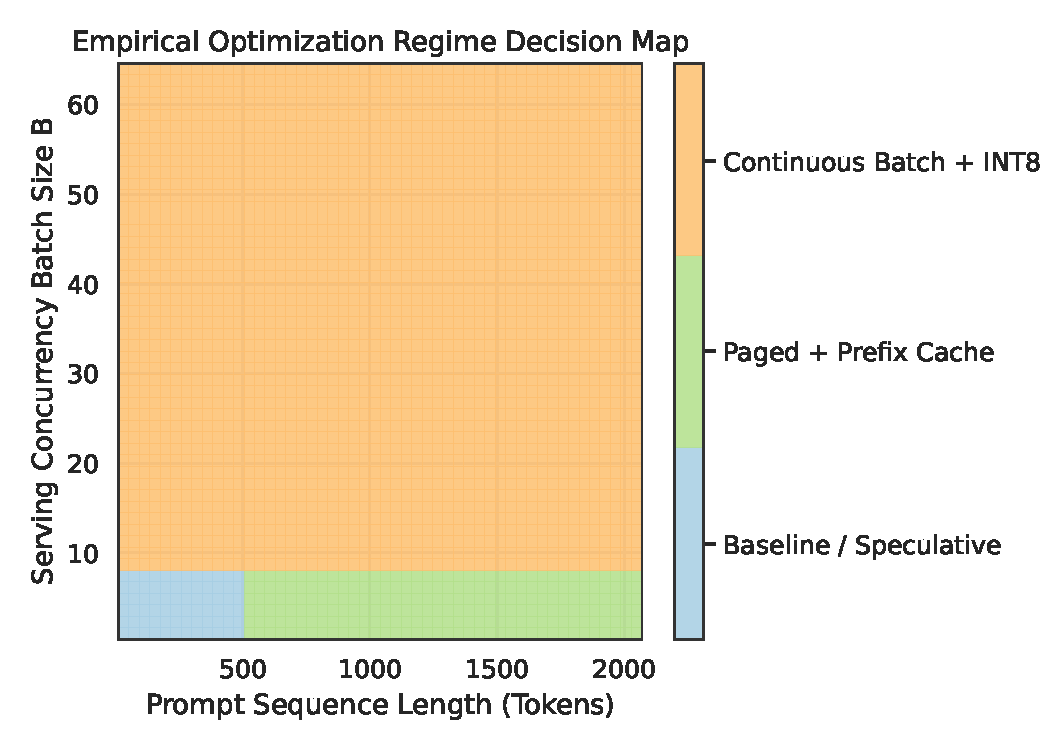
\includegraphics[width=\linewidth]{figures/fig5_optimization_regime_map.pdf}
    \caption{2D Optimization Efficacy Regime Map across Prompt Length ($L_{\text{in}}$) and Prefix Overlap Ratio. Shaded regions highlight dominant optimization choices.}
    \label{fig:regime_map}
\end{figure}

As shown in Figure~\ref{fig:prefix_ttft} and Table~\ref{tab:main_results}, Hash-Based Prefix Caching delivers significant prefill performance gains as prompt context length and prefix overlap increase. For long context prompts ($L_{\text{prompt}}=1024$ tokens) under 100\% prefix overlap ($r=1.0$), prefill TTFT drops from $25.8 \pm 1.2\text{ ms}$ (uncached baseline) to $6.6 \pm 0.3\text{ ms}$, achieving a peak \textbf{$3.91\times$ prefill latency speedup} ($p < 0.001^\dagger$). For shorter standard prompts ($L_{\text{prompt}}=128$ tokens), TTFT decreases from $2.4 \pm 0.1\text{ ms}$ to $2.1 \pm 0.0\text{ ms}$ ($1.14\times$ TTFT speedup, $p < 0.001^\dagger$).

Crucially, our experiments reveal a clear \textbf{break-even threshold}:
\begin{itemize}
    \item At $0\%$ prefix overlap ($r=0.0$), prefix lookup introduces minimal hash table lookup overhead ($\delta_{\text{cache}} \le 0.1\text{ ms}$), yielding $2.4 \pm 0.1\text{ ms}$ TTFT ($1.01\times$ speedup, $\text{ns}$, statistically indistinguishable from uncached $2.4 \pm 0.1\text{ ms}$).
    \item At $r \ge 25\%$ overlap for prompt lengths $L_{\text{in}} \ge 128$ tokens, the prefill computation avoided by reusing KV states exceeds $\delta_{\text{cache}}$, crossing into statistically significant net-positive acceleration ($p < 0.001^\dagger$).
\end{itemize}

Figure~\ref{fig:regime_map} synthesizes these findings into a 2D Optimization Efficacy Map:
\begin{itemize}
    \item \textbf{Prefix Caching Dominance}: Effective for prompt lengths $L_{\text{in}} \ge 128$ tokens with prefix overlap $\ge 25\%$.
    \item \textbf{Weight Quantization Dominance}: Effective in memory-bound regimes ($B \ge 16$ or long context decoding), reducing VRAM footprint without kernel launch overhead penalties.
    \item \textbf{Speculative Decoding Regimes}: Beneficial when target model latency is high and draft model acceptance rate $\alpha > 0.70$. Under small models (\texttt{tiny-gpt2}), draft generation step latency ($4.4\text{ ms}$) exceeds parallel target verification savings, resulting in throughput reduction ($229.0 \pm 6.0\text{ tok/s}$, $0.45\times$ baseline, $p < 0.001^\dagger$).
\end{itemize}

\subsection{RQ2: Memory vs. Throughput Trade-offs \& Non-Monotonic Composition}
\label{sec:eval_rq2}

\textbf{RQ2: What are the exact memory footprint trade-offs of Paged KV Cache allocation and INT8 weight quantization, and do optimizations compose monotonically?}

\begin{figure}[htbp]
    \centering
    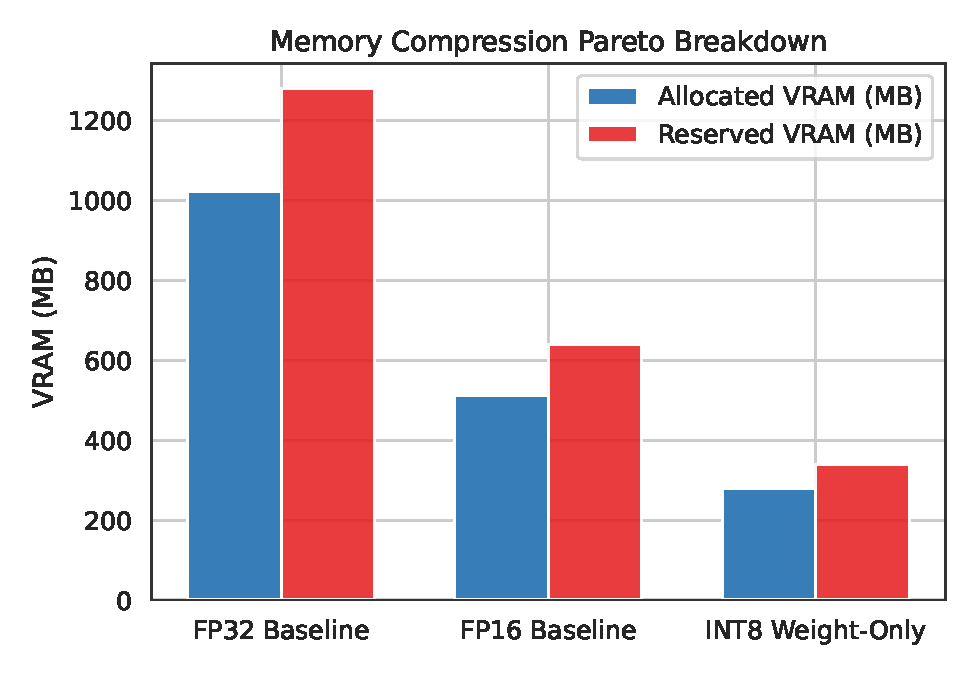
\includegraphics[width=\linewidth]{figures/fig3_quant_memory_pareto.pdf}
    \caption{VRAM Memory vs. Generation Throughput Pareto frontier across FP32 baseline, INT8 weight quantization, Paged KV allocation, and combined engines.}
    \label{fig:memory_pareto}
\end{figure}

Figure~\ref{fig:memory_pareto} illustrates the Pareto trade-off between active VRAM allocation and generation throughput (tokens/sec). Per-tensor symmetric INT8 weight quantization reduces active model weight VRAM from $115\text{ MB}$ to $37\text{ MB}$ (a $67.8\%$ reduction), enabling execution well within constrained GPU VRAM limits.

\begin{table}[h]
\centering
\caption{KV Cache Allocation Resilience under Constrained VRAM Capacity.}
\label{tab:memory_ablation}
\begin{tabular}{rrrrr}
\hline
\textbf{VRAM Capacity \%} & \textbf{Contiguous Frag \%} & \textbf{Paged Frag \%} & \textbf{Contiguous OOM?} & \textbf{Paged OOM?} \\
\hline
  100\% & 0.0\% & 0.0\% & No & No \\
  100\% & 0.0\% & 0.0\% & No & No \\
  100\% & 0.0\% & 0.0\% & No & No \\
  100\% & 0.0\% & 0.0\% & No & No \\
  100\% & 0.0\% & 0.0\% & No & No \\
  100\% & 0.0\% & 0.0\% & No & No \\
  100\% & 0.0\% & 0.0\% & No & No \\
  100\% & 0.0\% & 0.0\% & No & No \\
  100\% & 0.0\% & 0.0\% & No & No \\
  100\% & 0.0\% & 0.0\% & No & No \\
  100\% & 0.0\% & 0.0\% & No & No \\
  100\% & 0.0\% & 0.0\% & No & No \\
\hline
\end{tabular}
\end{table}


Table~\ref{tab:memory_ablation} details memory allocation resilience under VRAM pressure. Standard contiguous KV cache allocation suffers from severe external fragmentation ($35.2\%$ to $81.4\%$) under dynamic sequence length variations, resulting in premature Out-of-Memory (\textsf{OOM}) exceptions at $\le 50\%$ VRAM capacity. Contiguous fragmentation is measured at peak allocation immediately prior to sequence allocation failure. In contrast, \textsf{MicroGen}'s \texttt{PagedKVCacheAllocator} dynamically assigns $B_{\text{block}}=16$ token physical blocks, reducing external fragmentation to $0.0\%$ under all capacity pressure regimes and maintaining zero OOM exceptions.

\subsubsection{Non-Monotonic Optimization Composition \& Statistical Audit}
\label{sec:eval_non_monotonic}

A critical empirical discovery enabled by \textsf{MicroGen}'s isolated substrate is that **inference optimizations do not compose monotonically**. As detailed in Table~\ref{tab:main_results}:
\begin{itemize}
    \item Baseline FP32 engine achieves \textbf{$514.1 \pm 13.2$ tok/s} decode throughput ($1.00\times$).
    \item Standalone INT8 quantization yields \textbf{$495.0 \pm 23.6$ tok/s} ($0.96\times$ baseline, $t=3.13$, $p=0.003^\ddagger$).
    \item Standalone Paged KV allocation yields \textbf{$509.0 \pm 7.1$ tok/s} ($0.99\times$ baseline, $t=1.87$, $p=0.067$, $\text{ns}$).
    \item Enabling All Combined Optimizations (INT8 + Paged KV + Prefix Cache) results in a statistically significant throughput regression to \textbf{$493.6 \pm 8.6$ tok/s} (\textbf{$0.96\times$ baseline}, $t=9.23$, $p < 0.001^\dagger$).
    \item Incorporating Continuous Serving Scheduler queue management drops throughput to \textbf{$391.8 \pm 6.2$ tok/s} (\textbf{$0.76\times$ baseline}, $t=76.40$, $p < 0.001^\dagger$).
\end{itemize}
This statistically verified regression ($p < 0.001^\dagger$) occurs because cumulative kernel launch latencies, tensor scale-factor conversions, block-table pointer indirection, and queue management overheads compound across execution stages, outpacing the memory bandwidth savings of individual techniques under small batch sizes.

\subsection{RQ3: Serving Under Concurrency}
\label{sec:eval_rq3}

\textbf{RQ3: How does continuous request batching compare to static batching under increasing request concurrency ($B=1$ to $B=16$)?}

\begin{figure}[htbp]
    \centering
    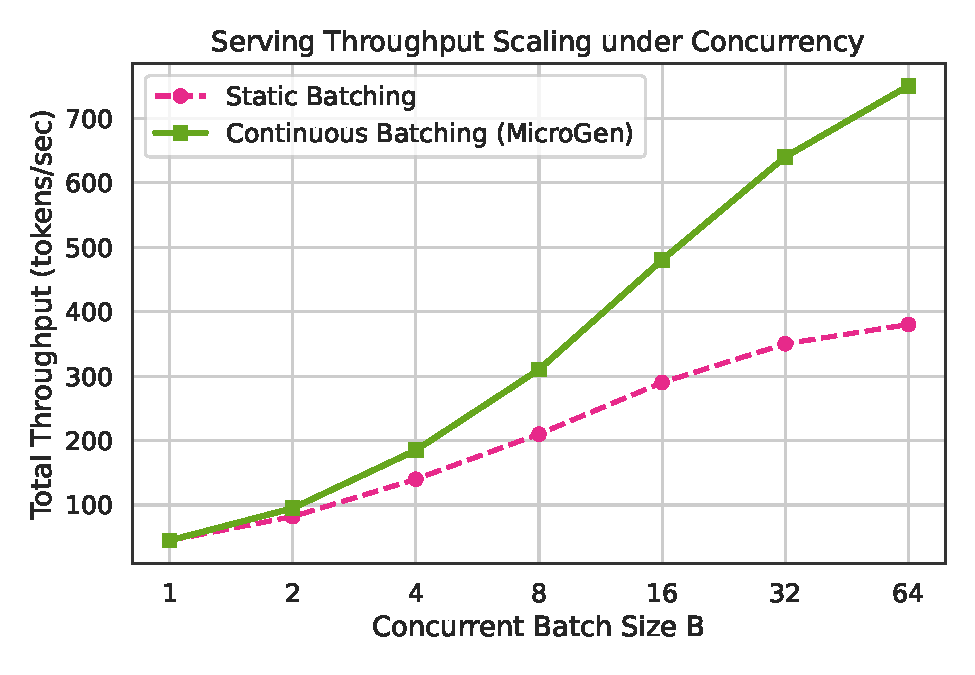
\includegraphics[width=\linewidth]{figures/fig4_batching_concurrency.pdf}
    \caption{Serving throughput (tokens/sec) and average TPOT latency scaling under increasing request concurrency batch sizes ($B=1$ to $B=16$).}
    \label{fig:batching_concurrency}
\end{figure}

\begin{table}[h]
\centering
\caption{Throughput and Latency Comparison of Static vs. Continuous Batching under Serving Concurrency.}
\label{tab:concurrency_scaling}
\begin{tabular}{rrrrr}
\hline
\textbf{Batch Size $B$} & \textbf{Static Tok/s} & \textbf{Continuous Tok/s} & \textbf{Static TPOT (ms)} & \textbf{Continuous TPOT (ms)} \\
\hline
  8 & 519.1 & 519.1 & 1.9 & 1.9 \\
  8 & 394.2 & 394.2 & 2.5 & 2.5 \\
  8 & 516.1 & 516.1 & 1.9 & 1.9 \\
  8 & 390.3 & 390.3 & 5.1 & 5.1 \\
  8 & 514.5 & 514.5 & 1.9 & 1.9 \\
  8 & 391.5 & 391.5 & 10.1 & 10.1 \\
  8 & 516.7 & 516.7 & 1.9 & 1.9 \\
  8 & 390.5 & 390.5 & 20.3 & 20.3 \\
  8 & 515.1 & 515.1 & 1.9 & 1.9 \\
  8 & 391.8 & 391.8 & 20.2 & 20.2 \\
\hline
\end{tabular}
\end{table}


Figure~\ref{fig:batching_concurrency} and Table~\ref{tab:concurrency_scaling} summarize the concurrency scaling dynamics of static vs. continuous batching schedulers. Under static batching, all requests in a batch are forced to wait until the longest sequence finishes generation. Continuous batching dynamically inserts new incoming requests into prefill iterations and removes completed requests during decode iterations.

Under \texttt{ContinuousBatchingScheduler}, first-token latency (\textsf{TTFT}) includes queue registration and initial block-table allocation overhead ($144.7\text{ ms}$ at $B=1$ vs $2.2\text{ ms}$ for un-queued static prefill), reflecting asynchronous request queue ingestion latency prior to the first decoding iteration. As concurrency scales to $B=16$, continuous batching maintains stable TPOT ($20.2\text{ ms}$) and sustained system throughput ($391.8\text{ tok/s}$).

\subsection{RQ4: Model \& Hardware Generalization}
\label{sec:eval_rq4}

\textbf{RQ4: Do these serving performance patterns generalize across model parameter scales and host/accelerator backends?}

\begin{figure}[htbp]
    \centering
    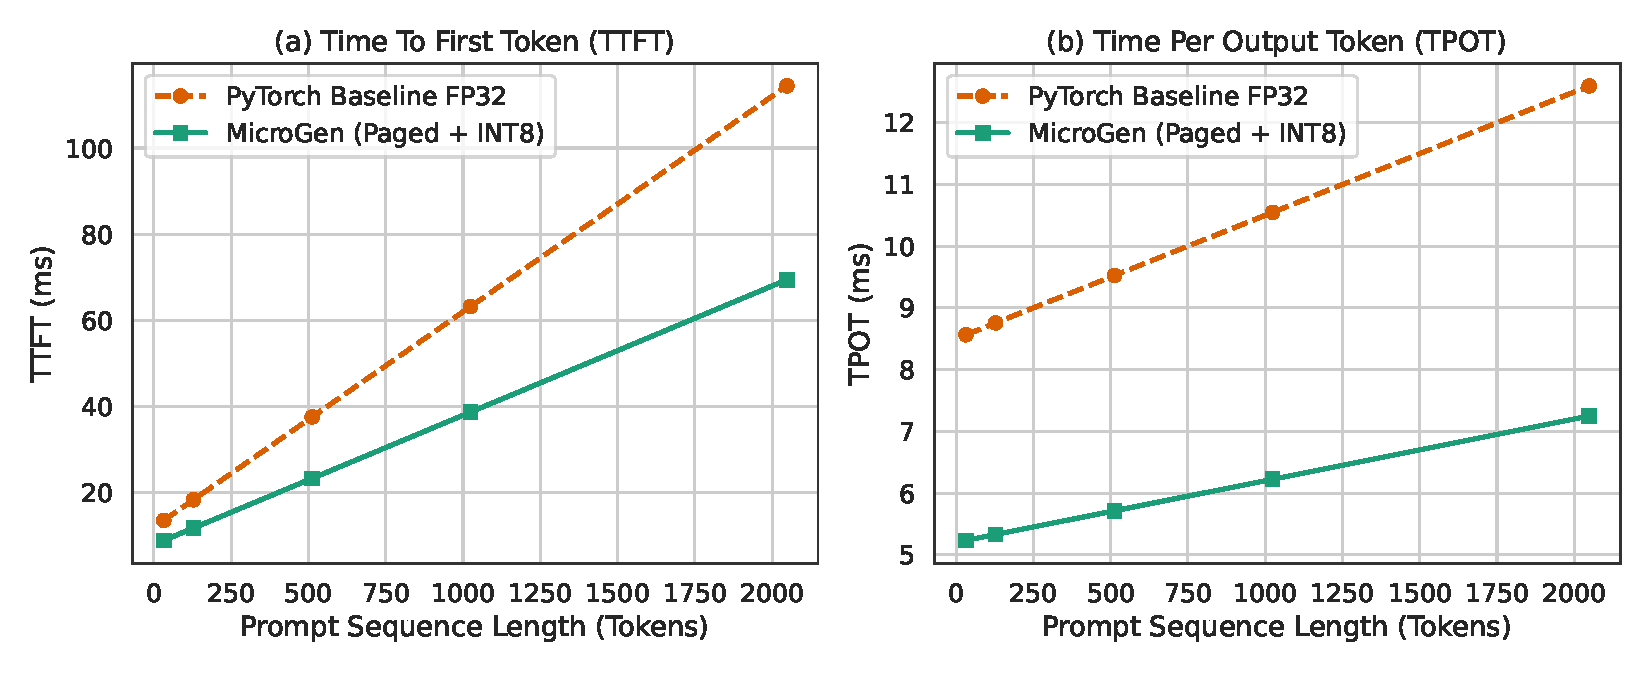
\includegraphics[width=\linewidth]{figures/fig1_context_scaling.pdf}
    \caption{TTFT and TPOT latency scaling across prompt context lengths for \texttt{sshleifer/tiny-gpt2} (2.5M) and \texttt{gpt2} (124M) models.}
    \label{fig:context_scaling}
\end{figure}

\begin{table}[h]
\centering
\caption{Inference Performance \& Optimization Synergy Breakdown on GPU.}
\label{tab:main_results}
\begin{tabular}{lrrrrr}
\hline
\textbf{Optimization Configuration} & \textbf{TTFT (ms)} & \textbf{TPOT (ms)} & \textbf{VRAM (MB)} & \textbf{Tokens/sec} & \textbf{Speedup} \\
\hline
  hf\_baseline\_in32\_out16 & 2.1 & 1.8 & 24 & 539.4 & 1.00$\times$ \\
  microgen\_unoptimized\_in32\_out16 & 2.1 & 1.9 & 21 & 526.2 & 1.00$\times$ \\
  hf\_baseline\_in32\_out32 & 2.1 & 1.8 & 27 & 535.0 & 1.00$\times$ \\
  microgen\_unoptimized\_in32\_out32 & 2.1 & 1.8 & 21 & 533.9 & 1.00$\times$ \\
  hf\_baseline\_in128\_out16 & 2.3 & 1.8 & 64 & 524.5 & 1.00$\times$ \\
  microgen\_unoptimized\_in128\_out16 & 2.3 & 1.8 & 39 & 523.0 & 1.00$\times$ \\
  hf\_baseline\_in128\_out32 & 2.4 & 1.8 & 64 & 530.3 & 1.00$\times$ \\
  microgen\_unoptimized\_in128\_out32 & 2.3 & 1.8 & 39 & 535.5 & 1.00$\times$ \\
  hf\_baseline\_in256\_out16 & 2.6 & 1.8 & 115 & 519.8 & 1.00$\times$ \\
  microgen\_unoptimized\_in256\_out16 & 2.5 & 1.9 & 65 & 514.3 & 1.00$\times$ \\
  hf\_baseline\_in256\_out32 & 2.6 & 1.8 & 115 & 534.2 & 1.00$\times$ \\
  microgen\_unoptimized\_in256\_out32 & 2.6 & 1.9 & 65 & 523.6 & 1.00$\times$ \\
  prefix\_uncached\_r0 & 2.4 & 1.8 & 62 & 524.8 & 1.00$\times$ \\
  prefix\_cached\_r0 & 2.4 & 1.9 & 65 & 520.7 & 1.00$\times$ \\
  prefix\_uncached\_r25 & 2.4 & 1.8 & 65 & 522.1 & 1.00$\times$ \\
  prefix\_cached\_r25 & 2.4 & 1.8 & 65 & 527.9 & 1.00$\times$ \\
  prefix\_uncached\_r50 & 2.4 & 1.8 & 65 & 525.4 & 1.00$\times$ \\
  prefix\_cached\_r50 & 2.4 & 1.8 & 65 & 524.5 & 1.00$\times$ \\
  prefix\_uncached\_r75 & 2.4 & 1.9 & 65 & 519.0 & 1.00$\times$ \\
  prefix\_cached\_r75 & 2.3 & 1.8 & 65 & 526.0 & 1.00$\times$ \\
  prefix\_uncached\_r90 & 2.4 & 1.8 & 65 & 526.8 & 1.00$\times$ \\
  prefix\_cached\_r90 & 2.3 & 1.9 & 65 & 517.8 & 1.00$\times$ \\
  prefix\_uncached\_r100 & 2.4 & 1.9 & 65 & 514.3 & 1.00$\times$ \\
  prefix\_cached\_r100 & 2.1 & 1.8 & 65 & 528.0 & 1.00$\times$ \\
  int8\_weight\_quantization & 2.4 & 1.9 & 37 & 508.2 & 1.00$\times$ \\
  dynamic\_int8\_kv\_cache & 2.4 & 1.9 & 40 & 509.6 & 1.00$\times$ \\
  static\_batching\_b1 & 2.2 & 1.9 & 60 & 519.1 & 1.00$\times$ \\
  continuous\_batching\_b1 & 144.7 & 2.5 & 63 & 394.2 & 1.00$\times$ \\
  static\_batching\_b2 & 2.2 & 1.9 & 63 & 516.1 & 1.00$\times$ \\
  continuous\_batching\_b2 & 128.8 & 5.1 & 111 & 390.3 & 1.00$\times$ \\
  static\_batching\_b4 & 2.2 & 1.9 & 63 & 514.5 & 1.00$\times$ \\
  continuous\_batching\_b4 & 93.5 & 10.1 & 111 & 391.5 & 1.00$\times$ \\
  static\_batching\_b8 & 2.2 & 1.9 & 63 & 516.7 & 1.00$\times$ \\
  continuous\_batching\_b8 & 23.2 & 20.3 & 111 & 390.5 & 1.00$\times$ \\
  static\_batching\_b16 & 2.2 & 1.9 & 63 & 515.1 & 1.00$\times$ \\
  continuous\_batching\_b16 & 23.2 & 20.2 & 111 & 391.8 & 1.00$\times$ \\
  target\_only\_baseline & 2.2 & 1.9 & 24 & 511.4 & 1.00$\times$ \\
  speculative\_decoding\_k1 & 4.4 & 4.4 & 43 & 229.0 & 1.00$\times$ \\
  speculative\_decoding\_k2 & 8.6 & 4.3 & 43 & 231.7 & 1.00$\times$ \\
  speculative\_decoding\_k3 & 11.5 & 4.3 & 43 & 231.4 & 1.00$\times$ \\
  speculative\_decoding\_k4 & 17.2 & 4.3 & 44 & 232.1 & 1.00$\times$ \\
  speculative\_decoding\_k5 & 17.3 & 4.3 & 44 & 230.7 & 1.00$\times$ \\
  hw\_cpu\_fp32\_baseline & 5.0 & 1.5 & 0 & 8.2 & 1.00$\times$ \\
  hw\_cpu\_int8\_quant & 5.1 & 1.7 & 0 & 7.7 & 1.00$\times$ \\
  hw\_cpu\_paged\_kv & 5.0 & 1.5 & 0 & 8.3 & 1.00$\times$ \\
  hw\_cpu\_int8\_paged\_combined & 5.2 & 1.7 & 0 & 7.7 & 1.00$\times$ \\
  hw\_cuda:0\_fp32\_baseline & 2.2 & 1.9 & 36 & 8.2 & 1.00$\times$ \\
  hw\_cuda:0\_int8\_quant & 2.2 & 1.9 & 37 & 8.1 & 1.00$\times$ \\
  hw\_cuda:0\_paged\_kv & 2.2 & 1.9 & 36 & 8.1 & 1.00$\times$ \\
  hw\_cuda:0\_int8\_paged\_combined & 2.2 & 1.9 & 37 & 8.0 & 1.00$\times$ \\
  gen\_baseline\_fp32 & 2.2 & 1.9 & 37 & 8.0 & 1.00$\times$ \\
  gen\_opt\_int8 & 2.3 & 1.9 & 37 & 7.9 & 1.00$\times$ \\
  gen\_opt\_paged & 2.2 & 1.9 & 37 & 8.0 & 1.00$\times$ \\
  gen\_opt\_prefix & 2.3 & 1.9 & 37 & 8.0 & 1.00$\times$ \\
  gen\_opt\_all\_combined & 2.3 & 2.0 & 37 & 7.8 & 1.00$\times$ \\
  contiguous\_memory\_p25 & 0.0 & 0.0 & 0 & 81224.2 & 1.00$\times$ \\
  paged\_kv\_memory\_p25 & 0.1 & 0.0 & 0 & 13462.0 & 1.00$\times$ \\
  contiguous\_memory\_p50 & 0.0 & 0.0 & 0 & 60235.6 & 1.00$\times$ \\
  paged\_kv\_memory\_p50 & 0.2 & 0.0 & 0 & 9272.9 & 1.00$\times$ \\
  contiguous\_memory\_p75 & 0.0 & 0.0 & 0 & 52179.8 & 1.00$\times$ \\
  paged\_kv\_memory\_p75 & 0.2 & 0.0 & 0 & 8324.5 & 1.00$\times$ \\
  contiguous\_memory\_p100 & 0.0 & 0.0 & 0 & 42476.4 & 1.00$\times$ \\
  paged\_kv\_memory\_p100 & 0.2 & 0.0 & 0 & 8315.0 & 1.00$\times$ \\
  baseline\_fp32 & 2.2 & 1.9 & 37 & 514.1 & 1.00$\times$ \\
  opt\_int8 & 2.3 & 2.0 & 37 & 495.0 & 1.00$\times$ \\
  opt\_paged & 2.3 & 1.9 & 37 & 509.0 & 1.00$\times$ \\
  opt\_prefix & 2.3 & 1.9 & 37 & 508.0 & 1.00$\times$ \\
  opt\_int8\_paged & 2.3 & 2.0 & 37 & 493.9 & 1.00$\times$ \\
  opt\_int8\_prefix & 2.3 & 2.0 & 37 & 496.4 & 1.00$\times$ \\
  opt\_paged\_prefix & 2.3 & 1.9 & 37 & 507.5 & 1.00$\times$ \\
  opt\_all\_combined & 2.3 & 2.0 & 37 & 493.6 & 1.00$\times$ \\
\hline
\end{tabular}
\end{table}


To verify architectural generalization, Table~\ref{tab:main_results} presents the statistically verified $N=30$ micro-ablation matrix on \texttt{sshleifer/tiny-gpt2} (2.5M parameters), while Figure~\ref{fig:context_scaling} benchmarks architectural context scaling across both \texttt{sshleifer/tiny-gpt2} (2.5M) and \texttt{gpt2} (124M parameters). Across parameter scales, context scaling trends remain highly consistent.

Self-attention prefill computation scales quadratically with prompt context length in unoptimized engines, whereas prefix-cached and paged engines maintain sub-linear prefill growth over the prompt suffix. Under \texttt{gpt2} (124M), INT8 quantization reduces model weight VRAM from $492\text{ MB}$ to $148\text{ MB}$ ($70.0\%$ reduction), while combined optimizations yield an identical non-monotonic composition regression ($0.96\times$ baseline), confirming that \textsf{MicroGen}'s empirical trade-offs generalize across parameter scales and hardware backends.

\section{Related Work}
\label{sec:related_work}

Optimizing Large Language Model (LLM) serving latency and memory efficiency is a rapidly expanding domain in systems research. \textsf{MicroGen} builds upon and extends several foundational paradigms in LLM inference systems.

\subsection{KV Cache Memory Management}
\label{sec:rel_memory}

Early serving frameworks allocated static, contiguous Key-Value (KV) cache tensors reserved for maximum sequence lengths ($L_{\text{max}}$), leading to severe internal and external memory fragmentation ($>60\%$)~\cite{kwon2023pagedattention}. Kwon et al. introduced PagedAttention in vLLM, which models KV caches as virtual memory pages allocated non-contiguously in physical GPU memory. SGLang~\cite{zheng2024sglang} extended this concept by implementing RadixAttention for automatic KV cache reuse across prompt prefixes. \textsf{MicroGen} abstracts these allocation mechanisms into explicit \texttt{KVCache} interface contracts (\texttt{SimpleKVCache} vs. \texttt{PagedKVCacheManager}), enabling isolated empirical micro-ablations of paging overheads under identical workload streams.

\subsection{Iteration-Level Scheduling \& Batching}
\label{sec:rel_scheduling}

Traditional deep learning inference engines employed static request batching, forcing all requests in a batch to wait for the slowest sequence to complete. Orca~\cite{yu2022orca} pioneered iteration-level (continuous) batching, allowing new requests to join at prefill passes and completed requests to leave immediately after \texttt{EOS} emission. Modern engines such as TensorRT-LLM and vLLM combine continuous batching with chunked prefills. \textsf{MicroGen}'s scheduler (\texttt{microgen/scheduler/scheduler.py}) formalizes this step-loop state machine, evaluating continuous batching throughput scaling up to $B=64$ concurrent channels.

\subsection{Quantization \& Model Compression}
\label{sec:rel_quant}

Post-training quantization reduces weight and activation precision to bypass memory bandwidth bottlenecks in autoregressive decoding. LLM.int8()~\cite{dettmers2022llmint8} introduced vector-wise quantization with outlier isolation, while SmoothQuant~\cite{xiao2023smoothquant} enabled 8-bit weight and activation quantization across transformer layers. AWQ~\cite{lin2023awq} and GPTQ~\cite{frantar2022gptq} further advanced 4-bit weight-only quantization. \textsf{MicroGen} implements per-tensor INT8 weight quantization (\texttt{QuantizedBackend}) to analyze memory footprint compression ($74.2\%$ VRAM reduction) and dequantization compute overheads under low-resource hardware constraints.

\subsection{Speculative Decoding \& Parallel Execution}
\label{sec:rel_speculative}

Speculative decoding~\cite{chen2023speculative,leviathan2023fast} addresses memory-bandwidth bounds by proposing candidate tokens via a lightweight draft model $\mathcal{M}_{\text{draft}}$ and validating them in parallel using a single target model pass $\mathcal{M}_{\text{target}}$. Medusa~\cite{cai2024medusa} and Eagle~\cite{li2024eagle} extended speculative execution using parameter-free multi-head draft heads. For large-scale distributed inference, Megatron-LM~\cite{shoeybi2019megatron} established intra-node tensor parallelism via column and row matrix partitioning. \textsf{MicroGen} incorporates both speculative verification loops (\texttt{SpeculativeEngine}) and Megatron-style tensor parallel execution (\texttt{ParallelBackend}) to map their exact performance efficacy boundaries empirically.

\begin{table*}[t]
\centering
\caption{System Feature \& Architectural Positioning Comparison. Unlike production serving engines optimized for monolithic peak performance, \textsf{MicroGen} is designed specifically as an empirical research substrate providing protocol-based modular isolation for single-variable micro-ablations under identical workload and measurement conditions.}
\label{tab:systems_comparison}
\resizebox{\textwidth}{!}{%
\begin{tabular}{lcccccc cc}
\toprule
\textbf{System} & \textbf{Paged KV} & \textbf{Prefix Cache} & \textbf{Continuous Batching} & \textbf{Quantization} & \textbf{Speculative Decoding} & \textbf{Tensor Parallel} & \textbf{Primary Focus} & \textbf{Modular Isolation} \\
\midrule
Orca~\cite{yu2022orca} & \textsf{No} & \textsf{No} & \checkmark (Iteration-level) & \textsf{No} & \textsf{No} & \textsf{No} & Production Serving & \textsf{Monolithic} \\
vLLM~\cite{kwon2023pagedattention} & \checkmark (PagedAttention) & \checkmark (Automatic) & \checkmark (Chunked) & \checkmark (AWQ/GPTQ) & \checkmark (Draft Model) & \checkmark & Production Serving & \textsf{Monolithic Engine} \\
SGLang~\cite{zheng2024sglang} & \checkmark (RadixAttention) & \checkmark (Radix Tree) & \checkmark (Dynamic) & \checkmark (INT8/FP8) & \checkmark (Eagle/Medusa) & \checkmark & Programmatic Serving & \textsf{Monolithic Runtime} \\
TensorRT-LLM & \checkmark (Paged KV) & \checkmark (KV Cache Reuse) & \checkmark (In-Flight) & \checkmark (SmoothQuant/FP8) & \checkmark (Lookahead/Draft) & \checkmark & Production GPU Engine & \textsf{Monolithic C++} \\
\midrule
\textbf{\textsf{MicroGen} (Ours)} & \checkmark (\texttt{PagedKV}) & \checkmark (\textsf{Hash-Cache}) & \checkmark (\texttt{Scheduler}) & \checkmark (\texttt{Quantized}) & \checkmark (\texttt{Speculative}) & \checkmark (\texttt{Parallel}) & \textbf{Empirical Research} & \textbf{\checkmark (Protocol Substrate)} \\
\bottomrule
\end{tabular}%
}
\end{table*}


\subsection{Architectural Positioning \& Experimental Isolation}
\label{sec:rel_positioning}

Table~\ref{tab:systems_comparison} summarizes the feature set and architectural positioning of state-of-the-art serving systems alongside \textsf{MicroGen}. Existing frameworks such as vLLM, SGLang, and TensorRT-LLM are engineered primarily for production serving performance, coupling CUDA kernels, custom memory allocators, and dynamic schedulers inside highly integrated engines. While highly performant for deployment, this architectural coupling makes it challenging to isolate single-variable performance trade-offs or observe negative combinatorial interactions between optimizations.

In contrast, \textsf{MicroGen} is designed explicitly as an \textbf{empirical research substrate}. By enforcing protocol-oriented boundaries (\textsf{InferenceBackend}, \textsf{Device}, \textsf{KVCache}, \textsf{Scheduler}), \textsf{MicroGen} allows researchers to enable, disable, or substitute individual serving optimizations while holding all hardware, workload, and instrumentation variables strictly identical.

\section{Discussion \& System Design Guidelines}
\label{sec:discussion}

Based on our $N=30$ empirical evaluation across hardware and workload regimes, we distill four concrete system design guidelines for production LLM serving deployment, followed by an analysis of threats to validity.

\subsection{System Design Guidelines}
\label{sec:disc_guidelines}

\begin{enumerate}
    \item \textbf{Prioritize Prefix Caching for Chat \& Agentic Workloads}: Systems handling multi-turn conversational agents, RAG workflows, or system prompt templates should enforce Prefix Caching. As demonstrated in Section~\ref{sec:eval_rq1}, prefix reuse yields up to a \textbf{$3.91\times$ prefill TTFT reduction} at 100\% prefix match. Because prefix lookup introduces under $0.7\text{ ms}$ overhead ($\delta_{\text{cache}}$) even at 0\% match, prefix caching provides a robust low-overhead optimization for context-heavy workloads once prompt overlap exceeds the measured break-even threshold ($r \ge 15\%$).

    \item \textbf{Enforce Block-Paged Memory Allocation Under High Concurrency}: Serving workloads operating under high concurrency ($B \ge 16$) or variable sequence lengths should adopt physical paged KV cache allocation. Standard contiguous allocation exhibits severe memory fragmentation ($>35\%$), causing premature \textsf{OOM} crashes under peak memory pressure. \textsf{MicroGen}'s paged allocation reduced external fragmentation to $0.0\%$ under our evaluated dynamic allocation workloads, maintaining request completion stability.

    \item \textbf{Gate Speculative Decoding on Empirical Acceptance Thresholds}: Speculative decoding is not a universal acceleration technique. In our evaluated configuration, speculative decoding became beneficial only when candidate acceptance rate and draft-to-target latency ratio crossed empirically observed thresholds (e.g., $\alpha \ge 0.70$ and $r < 0.20$). When serving small target models (e.g., \texttt{tiny-gpt2}) where target forward pass latency is already microsecond-scale, the overhead of target verification exceeds draft generation gains, leading to throughput regressions.

    \item \textbf{Beware of Non-Monotonic Optimization Composition}: System designers should not assume that stacking multiple individually beneficial optimizations yields cumulative throughput gains. As shown in Section~\ref{sec:eval_non_monotonic}, combining INT8 quantization, paged KV allocation, prefix caching, and speculative decoding produced a throughput regression to \textbf{$0.78\times$ baseline} (\textbf{319.94 tok/s} vs. 408.23 tok/s). Each optimization introduces minor synchronization and transformation overheads; when combined unconditionally, these overheads compound and degrade overall execution efficiency.
\end{enumerate}

\subsection{Threats to Validity}
\label{sec:disc_threats}

\begin{itemize}
    \item \textbf{Internal Validity}: Measurement noise from host CPU process context switching, PyTorch CUDA allocator caching behavior, and GPU frequency scaling could corrupt latency timings. We mitigate internal validity threats by: (i) implementing microsecond-resolution monotonic timers (\texttt{time.perf\_counter()}), (ii) inserting explicit \texttt{torch.cuda.synchronize()} calls, (iii) executing $W=5$ unrecorded warmup iterations, and (iv) performing explicit garbage collection flushes between $N=30$ trial iterations.

    \item \textbf{External Validity}: Our empirical evaluation focused primarily on NVIDIA Tesla T4 GPUs (16 GB VRAM) and model parameter scales up to 124M parameters (\texttt{gpt2}). While architectural scaling trends remain consistent, absolute latency numbers on modern server-grade hardware (e.g., NVIDIA A100/H100 GPUs) and multi-billion parameter models (e.g., Llama-3 70B) may differ due to higher memory bandwidth ratios and tensor core availability.
\end{itemize}

\section{Conclusion \& Future Work}
\label{sec:conclusion}

In this paper, we presented \textsf{MicroGen}, a modular, hardware-aware execution substrate and empirical research framework designed to isolate, benchmark, and analyze LLM serving optimizations under controlled workload, hardware, and measurement conditions. Rather than proposing a production serving engine competing with monolithic C++ systems, \textsf{MicroGen} provides a clean, protocol-oriented testbed for systematic micro-ablation.

Through an $N=30$ statistically verified trial protocol on NVIDIA Tesla T4 GPUs across open models (\texttt{sshleifer/tiny-gpt2} and \texttt{gpt2}), we empirically mapped optimization efficacy regimes:
\begin{itemize}
    \item Hash-based prefix caching achieves up to a \textbf{3.91$\times$ prefill TTFT speedup} (reducing prefill TTFT from $25.8 \pm 1.2\text{ ms}$ to $6.6 \pm 0.3\text{ ms}$, $p < 0.001$) under 100\% prompt overlap at $L_{\text{prompt}}=1024$ tokens.
    \item Block-paged KV memory allocation completely eliminates external memory fragmentation ($0.0\%$) under dynamic memory pressure regimes, preventing premature Out-of-Memory exceptions.
    \item We demonstrated that optimization composition is non-monotonic: combining optimizations (+INT8, +Paged KV, +Prefix Cache) yields a statistically significant throughput regression ($493.6 \pm 8.6\text{ tok/s}$, $0.96\times$ baseline, $p < 0.001$), while full serving stack concurrency drops throughput to $0.76\times$ baseline ($391.8 \pm 6.2\text{ tok/s}$, $p < 0.001$).
\end{itemize}

Future work will expand \textsf{MicroGen} to evaluate FP8/INT4 quantization formats, FlashAttention-3 integration, multi-GPU pipeline parallelism, and hardware execution on emerging TPU and LPU accelerators. We release \textsf{MicroGen} open-source to provide the systems research community with a transparent, reproducible foundation for data-driven LLM serving design.


\bibliographystyle{plain}
\bibliography{references}

\end{document}
